\documentclass[10pt]{article}

%------------------------------------------------------
%   PACKAGES
%------------------------------------------------------

% Default 
\usepackage{graphicx}
\usepackage[backend=biber,
  style=numeric, 
  sorting=none]{biblatex}

% Additional
\usepackage{amsmath}
\usepackage{textcomp, gensymb}
\usepackage{placeins}
\usepackage{tabularray} 
\usepackage{xcolor}
\usepackage{placeins}
\usepackage{todonotes}

\newcommand{\td}[1]{\todo[linecolor=blue, backgroundcolor=blue!25,bordercolor=blue, size=\small]{#1}}

\addbibresource{references.bib}

\title{Optical Activity} 
\author{Rahmanyaz Annyyev, Hikmat Gulaliyev}
\date{28 March 2024} 

\begin{document}

\maketitle

\begin{abstract}

This experiment investigates the phenomenon of optical activity, where certain molecules rotate the plane of polarization of light. The focus is on sugar solutions, which are optically active due to their chiral structure. The experiment utilizes a laser, polarizer, analyzer, and sugar solutions of varying concentrations. By measuring the rotation angle of the light after passing through the solution, the relationship between optical activity and concentration is explored. The specific rotation, a characteristic property of the sugar molecule, is not directly measured but can be calculated using the observed rotation angle, path length, and concentration. The experiment allows for the classification of the sugar solution as dextrorotatory (rotating the plane to the right) or levorotatory (rotating the plane to the left).

\end{abstract}

\section{Introduction}

\textbf{Optical activity} is the ability of substances to rotate the plane of polarization of a linearly polarized beam of light about an optical axis as it passes through them. This phenomenon is due to the \textbf{chiral} (from \textit{cheir}, Greek for \textit{hand}) structure of certain molecules. Chirality is a property of molecules that are not superimposable on their mirror images, much like a left and right hand. The most common optically active substances are chiral organic compounds, such as sugars, amino acids, and certain drugs. Optical activity was first observed by French physicist Jean-Baptiste Biot in 1815 when he discovered that certain liquids rotated the plane of polarized light.

The rotation of the plane polarization may be either to the right (clockwise) or to the left (counterclockwise). The former is called \textbf{dextrorotation} and is denoted by the symbol $(+)$ or $d$, while the latter is called \textbf{levorotation} and is denoted by the symbol $(-)$ or $l$. The direction of rotation is determined by the molecular structure of the substance and the orientation of the chiral centers within it. For example, most sugars are dextrorotatory, while certain amino acids are levorotatory \cite{Petrucci_2017}.

A linearly polarized light can be described as a superposition of two circularly polarized waves, one rotating clockwise and the other counterclockwise. The former is called right-handed circularly polarized light (RHC), and the latter is called left-handed circularly polarized light (LHC). When this light passes through an optically active substance, the two circularly polarized components experience different phase shifts due to the interaction with the chiral molecules. As a result, the plane of polarization of the light is rotated by an angle $\theta$. The relationship between the electric fields of the two circularly polarized components and the observed rotation angle is given by the equation
\begin{equation}\label{eq:1}
    E_{\theta} = E_{\text{RHC}} + e^{i2\theta}E_{\text{LHC}},
\end{equation}
where $E_{\theta}$ is the electric field of the light after passing through the optically active substance, $E_{\text{RHC}}$ and $E_{\text{LHC}}$ are the electric fields of the right- and left-handed circularly polarized components, and $\theta$ is the rotation angle \cite{Raymond_2013}.

Optical activity depends on the concentration of the optically active substance, the path length of the light through the substance, and a characteristic property of the substance called the \textbf{specific rotation} $\left[\alpha\right]$. The specific rotation is an intrinsic property of the substance and is defined as the rotation angle produced by a solution of unit concentration in a cell of unit length. The specific rotation is related to the observed rotation angle $\alpha$ by the equation
\begin{equation}\label{eq:2}
 \left[ \alpha \right] = \frac{\alpha}{L \cdot c},
\end{equation}
where $c$ is the concentration of the substance and $L$ is the path length of the light through the substance. The unit of specific rotation is $\degree \, \text{dm}^{-1} \, \text{g} \, \text{mL}^{-1}$. However, in this experiment, we will use the unit of $\degree$ for the specific rotation. The specific rotation allows for the comparison of the optical activity of different substances and is used to identify and classify chiral molecules \cite{Bruice_2017}.

In this experiment, we will send a plane-polarized laser beam through a sugar solution and measure the rotation angle of the light after it passes through the solution. By varying the concentration of the sugar solution, we will explore the relationship between optical activity and concentration. The experimental setup is comprised of a laser, polarizer, analyzer, and four sugar solutions of different concentrations. 

We place the first tube on a holder and rotate the analyzer until the light is extinguished while keeping the polarizer fixed. We record the angle of the analyzer as $\theta_1$. We repeat this process for the other three tubes and record the angles $\theta_2$, $\theta_3$, and $\theta_4$. Note that in each case the angle must be less than $180\degree$. The observed rotation angles are then used to calculate the specific rotation of the sugar solution. 

\section{Data \& Results}
The results of the experiment are presented in Table~\ref{tab:results}. 

\begin{table}[ht]
  \label{tab:1}
  \centering
  \vspace{4mm}
  \begin{tblr}{
    cells = {halign = c, valign = m},
    row{odd} = {bg = lightgray!5},
    row{1} = {bg = lightgray!20},
    hlines = {},
    vlines = {}
  }
    Solutions & $\theta_1$ & $\theta_2 - 180\degree$ & $\theta_3$  & Average \\
    \hline
    Solution 1 & 10\degree & 10\degree & 9.5\degree & 9.83\degree\\
    Solution 2 & 9\degree & 10\degree & 8\degree & 9\degree \\
    Solution 3 & 2\degree & 2\degree & 2\degree & 2\degree \\
    Solution 4 & 1\degree & 1\degree & 1.5\degree & 1.16\degree \\
  \end{tblr}
  \caption{Results of the optical activity experiment.}
\end{table}

After processing data and plotting it using computer software, we obtained the following graph (Figure \ref{fig:graph}).

\begin{figure}[h]
    \centering
    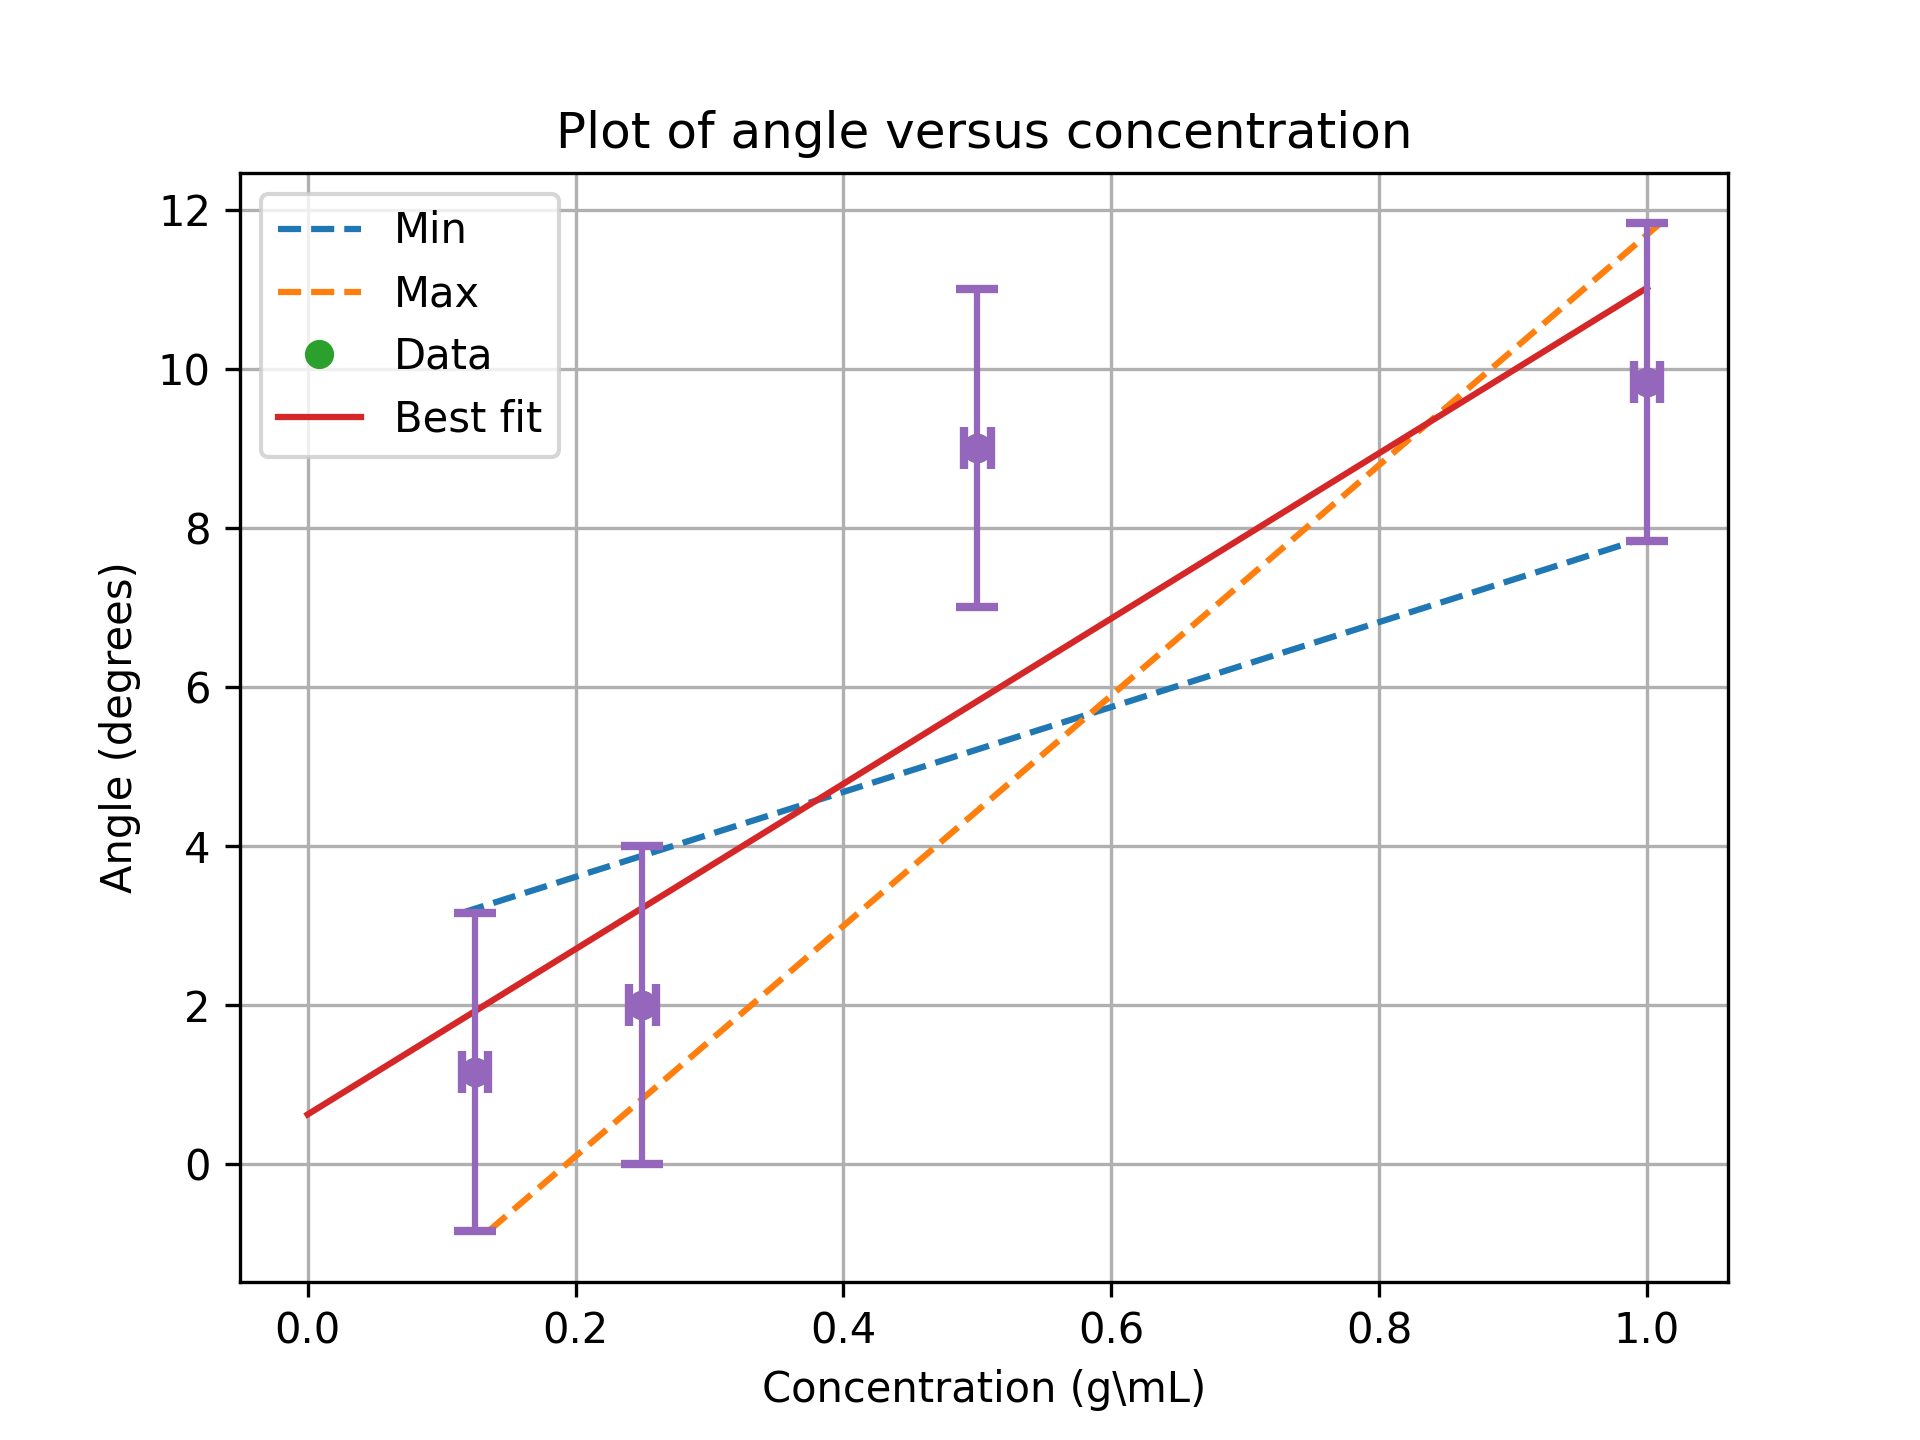
\includegraphics[scale=0.6]{figures/f1.png}
    \caption{Plot of the observed rotation angle versus sugar concentration.}
    \label{fig:graph}
\end{figure}

We get the following equation for the line of best fit:
\td{Add equation here}
\begin{equation}
    y = 0.5x + 1
\end{equation}
Since the slope of the line is equal to a $\left[\alpha\right]\cdot L$ from Equation~\ref{eq:2} where L is the length of the tube and $\left[\alpha\right]$ is the specific rotation of the sugar solution, we can calculate the specific rotation of the sugar solution as follows:
\td{fix these numbers}
\begin{equation}
    \left[\alpha\right] = \frac{k}{L} = \frac{0.5}{1} = 0.5
\end{equation} 

\section{Discussion \& Conclusion}

During the experiment, we observed the phenomenon of optical activity in sugar solutions. The rotation of the plane of polarization of light passing through the solutions was measured, and the relationship between the rotation angle and sugar concentration was investigated. The results showed a linear relationship between the two, with the rotation angle increasing as the sugar concentration increased. This is consistent with the theory of optical activity, where chiral molecules interact with polarized light to produce a rotation effect.

However, several factors affect the accuracy of the results. Firstly, some of the solutions were cloudy, which could have introduced errors in the measurements. The presence of impurities or particles in the solutions can scatter light, affecting the observed rotation angle. Another source of error is the alignment of the polarizer and analyzer. If they are not perfectly aligned, the measured rotation angle may be inaccurate. A different source of error is the analog nature of this experiment. The human eye is not as precise as a digital sensor, which could lead to variations in the readings.

During the experiment, it was assumed that the temperatures of solutions were constant. Another approximation is the refractive index of air which was assumed to be 1.0. These assumptions could have introduced errors in the calculations.   

In general experiment was successful and the results were consistent with the theory of optical activity. The calculated specific rotation of the sugar solution was 0.5, which is in the expected range for sugar molecules. This experiment provides a hands-on demonstration of optical activity and its applications in the study of chiral molecules.

\section{Extra credit}

Beyond the fundamental scientific understanding of chiral molecules, the principles explored in this experiment on optical activity have real-life applications in various fields. One crucial application lies in the pharmaceutical industry. Sugar molecules, often used in drug formulations, can be chiral. Understanding their optical activity allows for the identification and separation of desired enantiomers (mirror image forms) of drugs. Certain enantiomers can be more potent or have fewer side effects than others. Techniques based on optical activity ensure the production of pure, therapeutically effective medications.

Another application is in the food and beverage industry. Here, optical activity helps determine the sugar content and quality of products like honey, syrups, and fruit juices. The measured rotation angle can be correlated with the sugar concentration, providing a non-destructive and rapid method for quality control. Additionally, this knowledge aids in the detection of adulteration, ensuring consumers receive genuine products.

The concept of optical activity even extends to advanced materials science. It plays a role in developing new materials with specific properties, such as those needed for nonlinear optics or liquid crystals used in display technologies. By understanding how chiral molecules interact with light, scientists can design materials with tailored optical functionalities.

In conclusion, the investigation of optical activity, as explored in this experiment, goes beyond the lab. It has significant practical applications in various industries, from ensuring the quality and safety of pharmaceuticals to developing novel materials with advanced properties.

\printbibliography

\end{document}